\section{Ćwiczenia 1.}
\subsection{Zadanie. Pierwsza kwantyzacja - podstawowe pojęcia}
\textbf{uw}. Gaz doskonały to gaz elektronowy.\\\\
	\begin{itemize}
		\item Hamiltonian:
			\begin{equation} \underbrace{H(\r,\p)=\frac{p^2}{2m}}_{\text{mechanika klasyczna}} ~~\rightarrow~~ \underbrace{\hat{H}(\r,\p)=\frac{\hat{p}^2}{2m}}_{text{mechanika kwantowa}}\end{equation}
		\item Reprezentacja położeniowa:
		\begin{center}
			\begin{displaymath} \hat{x}=x \end{displaymath}
			\begin{displaymath} \hat{\r}=\r \end{displaymath}
			\begin{displaymath} \hat{\p}=-i\hbar\nabla \end{displaymath}
		\end{center}

		\item Zatem Hamiltonian ma postać:
			\begin{equation} \hat{H}=-\frac{\hbar^2}{2m}\nabla^2\end{equation}
		\item Algebra liniowa $\rightarrow$ równanie własne:\\
			Ogólnie:
			\begin{equation} \hat{A}\vec{x}=\lambda\vec{x}\end{equation}
			Dla hamiltonianu:
			\begin{equation}
			\hat{H}|~\Psi>~=~E|~\Psi>
			\end{equation}
	\item Funkcja falowa
			\begin{center}
			$~~~~~~~~~~\hat{H}|~\Psi>~=~E|~\Psi>~~~~~~~~~/\cdot<x|$\\
			$<x|\hat{H}|\Psi>~=~E<x|\Psi>$
			\end{center}	
			gdzie:
			\begin{equation} <x|\Psi>=\Psi(x)\end{equation}	
			to funkcja falowa. Jest ona określona jako współrzędna abstrakcyjna wektora stanu kwantowego względem ustalonej bazy (u nas - bazy położeniowej).
	\end{itemize}	
\subsection{Zadanie. Rozwiązanie równania Schroedingera dla cząstki swobodnej}
\begin{enumerate}
\item Wychodzimy od równania Schroedingera:
\begin{equation} \hat{H}\Psi(\r)=E\psi(\r)\end{equation}
czyli:
\begin{equation} \frac{\hbar^2}{2m}\nabla^2\Psi(\r)=E\psi(\r)\end{equation}
Rozwiązujemy je w pudle:\\
\begin{center}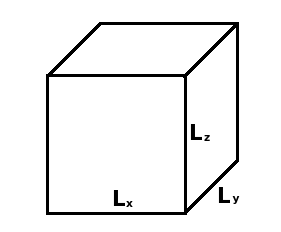
\includegraphics[scale=0.7]{obrazki/cwicz01_rys1.png}\end{center}
gdzie:
\begin{equation} L_i\rightarrow \infty\end{equation}
\item Postulujemy separację zmiennych:
\begin{equation}\Psi(\r)=X(x)Y(y)Z(z)\end{equation}
Laplasjan we współrzędnych kartezjańskich:
\begin{equation}\nabla^2=\frac{\partial^2}{\partial x^2}+\frac{\partial^2}{\partial y^2}+\frac{\partial^2}{\partial z^2}\end{equation}
Zatem równanie Schroedingera:
\begin{equation} -\Hc[Y(y)Z(z)X''(x)+X(x)Z(z)Y''(y)+X(x)Y(y)Z''(z)]=EX(x)Y(y)Z(z)~~~/:(XYZ)
\end{equation}
\begin{equation}-\Hc[\frac{X''(x)}{X(x)}+\frac{Y''(y)}{Y(y)}+\frac{Z''(z)}{Z(z)}]=E\end{equation}
X(x) wyliczymy następująco:
\begin{equation}-\Hc\frac{X''(x)}{X(x)}=E+\Hc[\frac{Y''(y)}{Y(y)}+\frac{Z''(z)}{Z(z)}]\end{equation}
\begin{equation} -\Hc\frac{X''(x)}{X(x)}=E_x\end{equation}
gdzie:
\begin{equation}E_x=E+\Hc[\frac{Y''(y)}{Y(y)}+\frac{Z''(z)}{Z(z)}]\end{equation}
Y(y) wyliczymy analogicznie:
\begin{equation}-\Hc\frac{Y''(y)}{Y(y)}=E+\Hc[\frac{X''(x)}{X(x)}+\frac{Z''(z)}{Z(z)}]\end{equation}
\begin{equation}-\Hc\frac{Y''(y)}{Y(y)}=E_y\end{equation}
gdzie:
\begin{equation}E_y=E-E_x+\frac{Z''(z)}{Z(z)}]\end{equation}
Z(z) również:
\begin{equation}-\Hc\frac{Z''(z)}{Z(z)}=E+\Hc[\frac{X''(x)}{X(x)}+\frac{Y''(y)}{Y(y)}]\end{equation}
\begin{equation}-\Hc\frac{Z''(z)}{Z(z)}=E_z\end{equation}
gdzie:
\begin{equation} E_z=E-E_x-E_y\end{equation}
\item Mamy zatem układ równań:\\
\begin{equation}
\begin{cases} 
-\Hc\frac{X''(x)}{X(x)}=E_x\\
-\Hc\frac{Y''(y)}{Y(y)}=E_y\\
-\Hc\frac{Z''(z)}{Z(z)}=E_z\\
E=E_x+E_y+Z_zz\\
\end{cases}
\end{equation}
gdzie ostatnie równanie to równanie więzów.\\
\item Rozwiązanie X(x)\\
To kombinacja liniowa:
\begin{equation} X(x)=A_1 e^{ik_xx}+A_2 e^{-ik_xx}\end{equation}
Z warunkiem brzegowym:
\begin{equation} X(0)=X(L_x)=0\end{equation}
Zatem:
\begin{equation}
\begin{cases}
X(0)=A_1+A_2=0 \\
X(L_x)=A_1 e^{ik_xL_x}+A_2 e^{-ik_xL_x}=0
\end{cases} \label{War.brzeg}
\end{equation}
Co można zapisać jako:
\begin{displaymath}
	 \left( \begin{array}{cc}
		1 & 1  \\
		 e^{ik_xL_x} & e^{-ik_xL_x} \\
	\end{array} \right)
	 \left( \begin{array}{c}
		A_1  \\
		A_2 \\
	\end{array} \right) 
	=
	\left( \begin{array}{c}
		0 \\
		0 \\
	\end{array} \right) 
\end{displaymath}
Dostaliśmy więc równanie macierzowe typu:
\begin{equation} M\vec{A}=\vec{0} \end{equation}
Rozwiązaniem tego równania jest:
\begin{equation} det M=0 \end{equation}
\begin{equation} e^{-ik_xL_x} - e^{ik_xL_x} =0 \end{equation}
\begin{equation} cos(k_xL_x)-isin(k_xL_x)-( cos(k_xL_x)+isin(k_xL_x))=0 \end{equation}
\begin{equation} -2isin(k_xL_x)=0 \end{equation}
Rozwiązaniem powyższego równania jest:
\begin{equation} k_xL_x=\pi n_x \end{equation}
gdzie:
\begin{equation}n_x \epsilon \mathbb{Z}\end{equation}
Ponieważ jednak:
\begin{equation} k_x>0~~\wedge~~L_x>0\end{equation}
to ostatecznie:
\begin{equation}k_xL_x=\pi n~~~,n=1,2,3,...\label{kwantowanie_k}\end{equation}

\item Rozwiązanie Y(y), Z(z)- analogicznie
\item Skwantowanie wektora falowego\\
Z równania (\ref{kwantowanie_k}) wynika \textbf{skwantowanie wektora falowego $k_n$}:
\begin{equation} k_{nx}=\frac{\pi n}{L_x}\end{equation}
Ogólnie:
\begin{equation} k_{ni}=\frac{\pi n}{L_i}~~~,i=x,y,z \label{k_wzor}\end{equation}

\item Energia
\begin{itemize}
	\item dla 1 zmiennej:
\begin{equation}E_{nx}=-\Hc\frac{X''}{X}=-\Hc(\frac{A_1(ik_x)^2e^{ik_xx}}{A_1e^{ik_xx}}+\frac{A_2(-ik_x)^2e^{-ik_xx}}{A_2e^{-ik_xx}})=\Hc k_x^2
\end{equation}
Po podstawieniu wyrażenia (\ref{k_wzor}), dostajemy:
\begin{equation}E_{nx}=\Hc (\frac{\pi n_x}{L_x})^2=\end{equation}
	\item Ogólnie:
\begin{equation}E_{n_xn_yn_z}=E_{nx}+E_{ny}+E_{nz}=\Hc(k_x^2+k_y^2+k_z^2)
\end{equation}
	\end{itemize}
	
\item Konsekwencje skwantowania wektora falowego $\vec{k}$ w przestrzeni wektora falowego.
Ponieważ wektor $\vec{k}$ jest skwantowany, to kolejne stany cząstki, czyli kolejne wartości $\vec{k}$ to punkty na siatce, pokazane schematycznie (w 2D) na rysunku pokazanym poniżej.\\
\begin{center}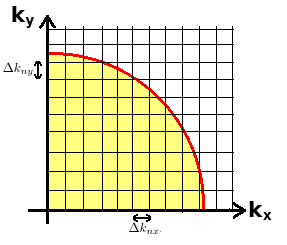
\includegraphics[scale=1]{obrazki/cwicz01_rys2.png}\end{center}
Taka siatka wyznacza sześciany. Można powiedzieć, że  na 1 stan w przestrzeni wektora $\vec{k}$ przypada sześcian o bokach:
\begin{equation} \Delta k_{ni}=k_{(n+1)i}-k_{ni}=\frac{\pi(n+1)}{L_i}-\frac{\pi n}{L_i}=\frac{\pi}{L_i} \end{equation}
czyli objętości:
\begin{equation}v_k=\Delta k_{nx}\Delta k_{ny}\Delta k_{nz}=\frac{\pi^3}{L_xL_yL_z}=\frac{\pi^3}{V}
\end{equation}
Jest to tzw. \textbf{objętość na 1 stan}.\\
Wszystkie dozwolone stany cząstki zajmują w przestrzeni wektora falowego pewien obszar. Gdyby n było całkowite, byłaby to cała kula. Jednak n jest naturalne, dlatego jest to $\frac{1}{8} kuli$, co również pokazano na powyższym rysunku.
Objętość tej części kuli, czyli objętość zajmowana przez wszystkie dozwolone stany cząstki, wynosi:
\begin{equation} V_k=\frac{1}{8}\cdot\frac{4}{3}\pi k^3=\frac{1}{6}\pi k^3
\end{equation}

\item Konsekwencje skwantowania wektora falowego $\vec{k}$ - liczba dozwolonych stanów N
Liczbę dozwolonych stanów możemy uzyskać poprzez podzielenie objętości wszystkich stanów przez objętość 1 stanu.\\
Biorąc pod uwagę jeszcze spin,\textbf{ liczba stanów} wyraża się wzorem:
\begin{equation} N=(2\sigma+1)\frac{V_k}{v_k} \end{equation}
gdzie: $(2\sigma+1)$ to rzut spinu.\\
 Dla elektronu:
\begin{equation}\sigma=\frac{1}{2}\end{equation}
zatem:
\begin{equation} N=2\frac{\frac{1}{6}\pi k^3}{\frac{\pi^3}{V}} = \frac{V}{3\pi^2}k^3\end{equation}
\item Konsekwencje skwantowania wektora falowego $\vec{k}$ - gęstość stanów DOS
Z definicji:
\begin{equation} DOS(E)=\rho(E)=\frac{dN(E)}{dE}\end{equation}
zatem musimy znaleźć związek N(E). Ponieważ zarówno N i E zależą od k, to wyliczymy:
\begin{equation}E=\frac{(\hbar k)^2}{2m}~~\Rightarrow~~k=\frac{\sqrt{2mE}}{\hbar}\end{equation}
\begin{equation}N= \frac{V}{3\pi^2}k^3=\frac{V}{3\pi^2}(\frac{{2mE}}{\hbar^2})^{3/2} \end{equation}
Zatem:
\begin{equation} DOS(E)=\rho(E)=\frac{dN}{dE}=\underbrace{\frac{V}{2\pi^2}(\frac{2m}{\hbar^2})^{3/2}}_{const.}E^{1/2}=CE^{1/2}\end{equation}
\end{enumerate}

\subsection{Zadanie Domowe}
Obliczyć całkę:
\begin{equation}\int_0^\mu \rho(E)E dE\end{equation}
\begin{equation}\int_0^\mu CE^{3/2} dE=\frac{2}{5}C\mu^{5/2}\end{equation}

